%\VignetteIndexEntry{Oligo Vignette}
%\VignetteDepends{oligo}
%\VignetteKeywords{Expression, SNP, Affymetrix, NimbleGen, Oligonucleotide Arrays}
%\VignettePackage{oligo}
\documentclass{article}

\newcommand{\Rfunction}[1]{{\texttt{#1}}}
\newcommand{\Rmethod}[1]{{\texttt{#1}}}
\newcommand{\Rcode}[1]{{\texttt{#1}}}
\newcommand{\Robject}[1]{{\texttt{#1}}}
\newcommand{\Rpackage}[1]{{\textsf{#1}}}
\newcommand{\Rclass}[1]{{\textit{#1}}}
\newcommand{\oligo}{\Rpackage{oligo }}

\usepackage{graphicx}

\usepackage{/home/bst/student/bcarvalh/bin/R-2.5.0/share/texmf/Sweave}
\begin{document}
\title{An Introduction to the Oligo Package}
\date{March, 2007}
\author{Benilton Carvalho}
\maketitle


\section{Introduction}

The \oligo package is designed to support all microarray designs
provided by Affymetrix and NimbleGen: expression, tiling, SNP and exon
arrays. With the increase in the density of the current technologies,
\oligo uses the resources offered by the \Rpackage{BufferedMatrix}
packages to handle the feature-level information. As of now,
chip-specific packages are built via \Rpackage{makePlatformDesign} and
transitioning to the \Rpackage{pdInfoBuilder} package, which creates
the data packages for the Affymetrix SNP arrays.

\section{Analyzing Affymetrix SNP Arrays}

Genotyping can be performed using \oligo and you will need:

\begin{itemize}
\item \oligo and its dependencies;
\item Chip specific data package, eg. \Rpackage{pd.mapping50k.xba240}:
  package that contains the array specifications and SNP annotation.
\item CEL files.
\end{itemize}

Figure \ref{workflow} shows the general workflow for genotyping using
the \oligo package. 

\begin{figure}[h]
  \centering
  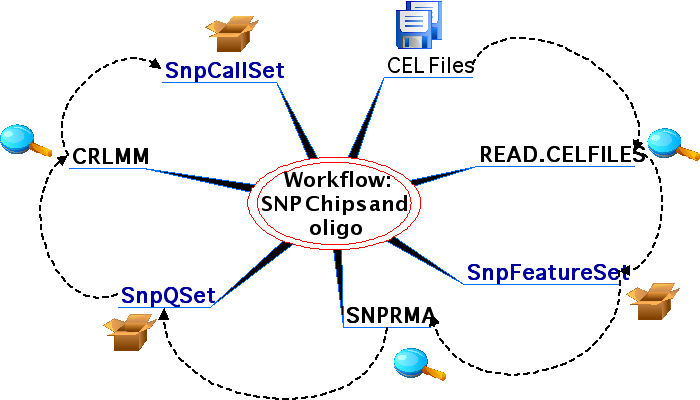
\includegraphics[scale=.5]{workflow.png}
  \caption{Genotyping workflow using the \oligo package.}
  \label{workflow}
\end{figure}

We will start by loading the \oligo package and importing the CEL
files available on the \Rpackage{sampleDataAffy100K}. The intensity
matrix will be a \Rclass{BufferedMatrix} object and this will require
the use of temporary files in order to reduce the RAM usage. Although
the temporary files can be stored anywhere, a better approach will be
to use a local directory rather than using a directory on the
network. The \Robject{tmpdir} in the \Rfunction{read.celfiles()} sets
the directory where the temporary files are going to be stored.

\begin{Schunk}
\begin{Sinput}
R> library(oligo)
R> library(hapmap100kxba)
R> pathCelFiles <- system.file("celFiles", package = "hapmap100kxba")
R> fullFilenames <- list.celfiles(path = pathCelFiles, 
     full.names = TRUE)
R> temporaryDir <- tempdir()
R> rawData <- read.celfiles(fullFilenames, tmpdir = temporaryDir)
\end{Sinput}
\begin{Soutput}
Incompatible phenoData object. Created a new one.


Welcome to the pd.Mapping50K_Xba240 prototype pdInfo package
WARNING: DO NOT USE THIS PACKAGE FOR ANY ANALYSIS.
THIS PACKAGE IS FOR INTERFACE PROTOTYPE USE ONLY!
THE DATA HAS NOT BEEN VALIDATED AND LIKELY HAS ERRORS.
Have fun!
\end{Soutput}
\end{Schunk}

The \Robject{rawData} object is of class \Rclass{SnpFeatureSet}, which
extends \Rclass{eSet}. Methods like \Rmethod{exprs()} and
\Rmethod{pm()} are defined and, again, return \Rclass{BufferedMatrix}
objects.

The \Rclass{phenoData} slot includes covariates about the
samples. Genotyping and copy number analyses often make use of gender
information in order to provide more precise inferences. The code
below exemplifies the creation of the \Rclass{phenoData} object.

\begin{Schunk}
\begin{Sinput}
R> aboutSamples <- data.frame(gender = c("female", 
     "female", "male"))
R> rownames(aboutSamples) <- sampleNames(rawData)
R> aboutVars <- data.frame(labelDescription = "male/female")
R> rownames(aboutVars) <- "gender"
R> phenoData(rawData) <- new("AnnotatedDataFrame", 
     data = aboutSamples, varMetadata = aboutVars)
\end{Sinput}
\end{Schunk}

Preprocessing SNP arrays can be done by using the \Rfunction{snprma()}
method, described in \cite{Carvalho2006}. Once it is completed, an
\Rclass{SnpQSet} object is returned, which is the summarized data of the
\Robject{rawData} object above. An overview of the method is presented
at Figure \ref{snprma}.

\begin{figure}[h]
  \centering
  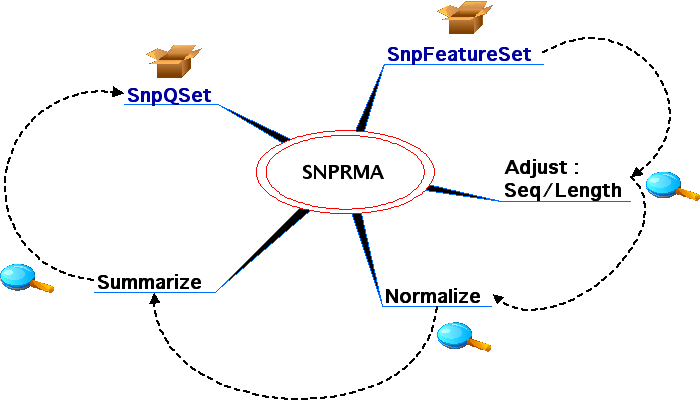
\includegraphics[scale=.5]{snprma.png}
  \caption{SNPRMA overview}
  \label{snprma}
\end{figure}

For each SNP there are four numbers $(\theta_{A-}, \theta_{B-},
\theta_{A+}, \theta_{B+})$, which are proportional to the
log-intensities in each of these combinations of allele and strand
($-$: antisense; $+$: sense). They are represented by four matrices:
\Robject{antisenseThetaA}, \Robject{antisenseThetaB},
\Robject{senseThetaA} and \Robject{senseThetaB}, which are the
components of the \Rclass{SnpQSet} object. One can extract these
objects using accessors of the same name.

Average intensities and log-ratios are defined as across allele and
within strand, ie:
\begin{eqnarray}
  A_{s} & = & \frac{\theta_{A, s}+\theta_{B, s}}{2} \\
  M_{s} & = & \theta_{A, s} - \theta_{B, s},
\end{eqnarray}
where $s$ defines the strand (antisense or sense). These quantities
can be obtained via \Rmethod{getA()} and \Rmethod{getM} methods, which
return high-dimensional arrays with dimensions corresponding to SNP's,
samples and strands, respectively.
\begin{Schunk}
\begin{Sinput}
R> preProcessedData <- snprma(rawData)
\end{Sinput}
\begin{Soutput}
This may take a while.
Adjusting for sequence and fragment length......... done.
Normalizing... done.
Calculating Expression
\end{Soutput}
\begin{Sinput}
R> theA <- getA(preProcessedData)
R> theM <- getM(preProcessedData)
R> dim(theA)
\end{Sinput}
\begin{Soutput}
[1] 58960     3     2
\end{Soutput}
\begin{Sinput}
R> str(theM)
\end{Sinput}
\begin{Soutput}
 num [1:58960, 1:3, 1:2] -0.0486  0.9062  0.9369  0.5323  2.0623 ...
 - attr(*, "dimnames")=List of 3
  ..$ : chr [1:58960] "SNP_A-1507972" "SNP_A-1510136" "SNP_A-1511055" "SNP_A-1518245" ...
  ..$ : chr [1:3] "CEU_NA06985_XBA.CEL.gz" "CEU_NA06991_XBA.CEL.gz" "CEU_NA06993_XBA.CEL.gz"
  ..$ : chr [1:2] "antisense" "sense"
\end{Soutput}
\end{Schunk}

These measures can be used, for example, to create an MA-plot and are
later used for genotyping. The example below generates an MA-plot for
the first sample using only the antisense strand data:
\begin{Schunk}
\begin{Sinput}
R> library(geneplotter)
R> smoothScatter(theA[, 1, 1], theM[, 1, 1], main = "MA-plot (Antisense)", 
     xlab = "Average Intensity", ylab = "Log-ratio (A/B)")
\end{Sinput}
\end{Schunk}
\includegraphics{oligo-maplot}

The CRLMM algorithm \cite{Carvalho2006} can be applied on a
\Rclass{SnpQSet} object in order to produce genotype calls. It involves
running a mixture of regressions via EM algorithm to adjust for average
intensity and fragment length in the log-ratio scale. These adjustments
may take long time to run, depending on the combination of number of
samples and computer resources available. To save time in subsequent
analyses, we must specify the name of the file that will store the
results obtained with the EM algorithm using the
\Robject{correctionFile} argument. If the file passed to
\Robject{correctionFile} does not exist, it is created, otherwise it is
loaded. Figure \ref{crlmm} presents a diagram of the CRLMM algorithm:

\begin{figure}[h]
  \centering
  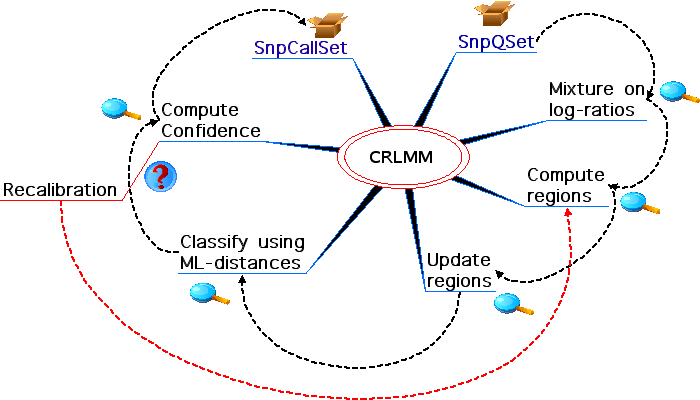
\includegraphics[scale=.5]{crlmm.png}
  \caption{CRLMM Algorithm diagram}
  \label{crlmm}
\end{figure}

\textbf{A word of warning}: the \Rmethod{crlmm()} method searches for a
variable \Robject{gender} in the \Rclass{phenoData} slot of the
\Rclass{SnpQSet} object. If it fails to find that variable, it will try
estimate the gender from the data. If there is not enough discrimination
power to estimate the gender, the following error message will be
returned:

{\bf empty cluster: try a better set of initial centers}

Increasing the sample size is one of the possible solutions, although
the preferred one is to have \Robject{gender} already defined in the
\Rclass{phenoData} slot.

\begin{Schunk}
\begin{Sinput}
R> crlmmOut <- crlmm(preProcessedData, correctionFile = "exampleCorrection.rda", 
     verbose = FALSE)
\end{Sinput}
\begin{Soutput}
Updating centers and scales.Done.
Computing confidence for calls on  3  arraysDone
Computing confidence for calls on  3  arraysDone
\end{Soutput}
\end{Schunk}

The \Robject{crlmmOut} object above belongs to the \Rclass{SnpCallSet}
class and contains the genotype calls and confidence measures
associated to the calls, represented respectively by the
\Robject{calls} and \Robject{callsConfidence} matrices. These matrices
can be accessed using the methods of the same name as demonstrated
below:

\begin{Schunk}
\begin{Sinput}
R> calls(crlmmOut)[1:5, 1:2]
\end{Sinput}
\begin{Soutput}
              CEU_NA06985_XBA.CEL.gz CEU_NA06991_XBA.CEL.gz
SNP_A-1507972                      2                      3
SNP_A-1510136                      1                      1
SNP_A-1511055                      1                      2
SNP_A-1518245                      2                      1
SNP_A-1641749                      1                      1
\end{Soutput}
\begin{Sinput}
R> callsConfidence(crlmmOut)[1:5, 1:2]
\end{Sinput}
\begin{Soutput}
              CEU_NA06985_XBA.CEL.gz CEU_NA06991_XBA.CEL.gz
SNP_A-1507972              0.9994679              0.9999017
SNP_A-1510136              0.9989516              0.9984237
SNP_A-1511055              0.9931806              0.9999105
SNP_A-1518245              0.9988607              0.9998467
SNP_A-1641749              0.9998194              0.9997692
\end{Soutput}
\end{Schunk}

The genotype calls are represented by 1 (AA), 2 (AB) and 3 (BB). The
confidence is the log-likelihood ratio of the two most likely calls.

\subsection{Exploring the Annotation Package}

The user who is willing to make deeper investigation using the
annotations provided for each SNP array can use SQL queries to access
more other information that might not be directly exposed.

The example below demonstrates how to see the available tables, fields
and extract chromosome, physical location and cytoband for the first
five SNP's (probes querying specific SNP's have names starting with
the string ``SNP'').

\begin{Schunk}
\begin{Sinput}
R> annot <- annotation(rawData)
R> conn <- db(get(annot))
R> dbListTables(conn)
\end{Sinput}
\begin{Soutput}
 [1] "featureSet"   "mmfeature"    "pm_mm"       
 [4] "pmfeature"    "qcmmfeature"  "qcpm_qcmm"   
 [7] "qcpmfeature"  "sequence"     "sqlite_stat1"
[10] "table_info"  
\end{Soutput}
\begin{Sinput}
R> dbListFields(conn, "featureSet")
\end{Sinput}
\begin{Soutput}
 [1] "fsetid"          "man_fsetid"      "affy_snp_id"    
 [4] "dbsnp_rs_id"     "chrom"           "physical_pos"   
 [7] "strand"          "allele_a"        "allele_b"       
[10] "fragment_length"
\end{Soutput}
\begin{Sinput}
R> sql <- "SELECT man_fsetid, chrom, physical_pos FROM featureSet WHERE man_fsetid LIKE 'SNP%' LIMIT 5"
R> dbGetQuery(conn, sql)
\end{Sinput}
\begin{Soutput}
     man_fsetid chrom physical_pos
1 SNP_A-1650338     2    168433267
2 SNP_A-1716667    19     40749462
3 SNP_A-1712945    19     53411226
4 SNP_A-1711654    21     31501701
5 SNP_A-1717655     1     15312743
\end{Soutput}
\end{Schunk}
 
\section{Details}

This document was written using:

\begin{Schunk}
\begin{Sinput}
R> sessionInfo()
\end{Sinput}
\begin{Soutput}
R version 2.5.0 (2007-04-23) 
x86_64-unknown-linux-gnu 

locale:
LC_CTYPE=en_US.UTF-8;LC_NUMERIC=C;LC_TIME=en_US.UTF-8;LC_COLLATE=en_US.UTF-8;LC_MONETARY=en_US.UTF-8;LC_MESSAGES=en_US.UTF-8;LC_PAPER=en_US.UTF-8;LC_NAME=C;LC_ADDRESS=C;LC_TELEPHONE=C;LC_MEASUREMENT=en_US.UTF-8;LC_IDENTIFICATION=C

attached base packages:
[1] "splines"   "tools"     "stats"     "graphics" 
[5] "grDevices" "utils"     "datasets"  "methods"  
[9] "base"     

other attached packages:
          geneplotter               lattice 
             "1.14.0"              "0.15-4" 
             annotate  pd.mapping50k.xba240 
             "1.14.1"               "0.1.5" 
        hapmap100kxba                 oligo 
                "1.0"               "1.0.5" 
BufferedMatrixMethods        BufferedMatrix 
              "1.0.0"               "1.0.0" 
              RSQLite                   DBI 
              "0.5-3"               "0.2-2" 
               affyio               Biobase 
              "1.4.0"              "1.14.0" 
\end{Soutput}
\end{Schunk}


\end{document}
